\documentclass[]{article}
\usepackage{amssymb,amsmath}
\usepackage{ifxetex,ifluatex}
\usepackage{fixltx2e} % provides \textsubscript
\ifxetex
  \usepackage{fontspec,xltxtra,xunicode}
  \defaultfontfeatures{Mapping=tex-text,Scale=MatchLowercase}
  \newcommand{\euro}{€}
\else
  \ifluatex
    \usepackage{fontspec}
    \defaultfontfeatures{Mapping=tex-text,Scale=MatchLowercase}
    \newcommand{\euro}{€}
  \else
    \usepackage[utf8]{inputenc}
  \fi
\fi
\usepackage{color}
\usepackage{fancyvrb}
\DefineShortVerb[commandchars=\\\{\}]{\|}
\DefineVerbatimEnvironment{Highlighting}{Verbatim}{commandchars=\\\{\}}
% Add ',fontsize=\small' for more characters per line
\newenvironment{Shaded}{}{}
\newcommand{\KeywordTok}[1]{\textcolor[rgb]{0.00,0.44,0.13}{\textbf{{#1}}}}
\newcommand{\DataTypeTok}[1]{\textcolor[rgb]{0.56,0.13,0.00}{{#1}}}
\newcommand{\DecValTok}[1]{\textcolor[rgb]{0.25,0.63,0.44}{{#1}}}
\newcommand{\BaseNTok}[1]{\textcolor[rgb]{0.25,0.63,0.44}{{#1}}}
\newcommand{\FloatTok}[1]{\textcolor[rgb]{0.25,0.63,0.44}{{#1}}}
\newcommand{\CharTok}[1]{\textcolor[rgb]{0.25,0.44,0.63}{{#1}}}
\newcommand{\StringTok}[1]{\textcolor[rgb]{0.25,0.44,0.63}{{#1}}}
\newcommand{\CommentTok}[1]{\textcolor[rgb]{0.38,0.63,0.69}{\textit{{#1}}}}
\newcommand{\OtherTok}[1]{\textcolor[rgb]{0.00,0.44,0.13}{{#1}}}
\newcommand{\AlertTok}[1]{\textcolor[rgb]{1.00,0.00,0.00}{\textbf{{#1}}}}
\newcommand{\FunctionTok}[1]{\textcolor[rgb]{0.02,0.16,0.49}{{#1}}}
\newcommand{\RegionMarkerTok}[1]{{#1}}
\newcommand{\ErrorTok}[1]{\textcolor[rgb]{1.00,0.00,0.00}{\textbf{{#1}}}}
\newcommand{\NormalTok}[1]{{#1}}
\usepackage{graphicx}
% We will generate all images so they have a width \maxwidth. This means
% that they will get their normal width if they fit onto the page, but
% are scaled down if they would overflow the margins.
\makeatletter
\def\maxwidth{\ifdim\Gin@nat@width>\linewidth\linewidth
\else\Gin@nat@width\fi}
\makeatother
\let\Oldincludegraphics\includegraphics
\renewcommand{\includegraphics}[1]{\Oldincludegraphics[width=\maxwidth]{#1}}
\ifxetex
  \usepackage[setpagesize=false, % page size defined by xetex
              unicode=false, % unicode breaks when used with xetex
              xetex,
              bookmarks=true,
              pdfauthor={},
              pdftitle={},
              colorlinks=true,
              urlcolor=blue,
              linkcolor=blue]{hyperref}
\else
  \usepackage[unicode=true,
              bookmarks=true,
              pdfauthor={},
              pdftitle={},
              colorlinks=true,
              urlcolor=blue,
              linkcolor=blue]{hyperref}
\fi
\hypersetup{breaklinks=true, pdfborder={0 0 0}}
\setlength{\parindent}{0pt}
\setlength{\parskip}{6pt plus 2pt minus 1pt}
\setlength{\emergencystretch}{3em}  % prevent overfull lines
\setcounter{secnumdepth}{0}


\begin{document}

\section{OceanColor Data Products and R}

This is a quick analysis and demo for downloading and importing global
oceancolor products (e.g SST, Chl-a) available from
\href{http://oceancolor.gsfc.nass.gov}{NASA's OceanColor Web} into R for
mapping and analysis. The steps and tools described here are only
guaranteed, at this point, to work within an OS X environment. That
said, the tools used are available for other platforms and should be
easily adapted.

\subsubsection{Required Software and Tools}

\begin{itemize}
\item
  R 2.15.0
\item
  GDAL 1.9 Complete frameworks available from
  \href{http://www.kyngchaos.com/software/frameworks}{KyngChaos}
\item
  rgdal 0.7.8-2 binary available from
  \href{http://www.kyngchaos.com/software/frameworks}{KyngChaos}
\item
  gdal programs must be available on the users path
\end{itemize}

\subsubsection{Load R Packages}

\begin{Shaded}
\begin{Highlighting}[]
\CommentTok{# if necessary uncomment and install packages.  install.packages('sp')}
\CommentTok{# install.packages('rgeos') install.packages('raster')}
\CommentTok{# install.packages('RCurl') install.packages('ggplot2')}
\KeywordTok{library}\NormalTok{(sp)}
\KeywordTok{library}\NormalTok{(rgdal)}
\KeywordTok{library}\NormalTok{(rgeos)}
\KeywordTok{library}\NormalTok{(raster)}
\KeywordTok{library}\NormalTok{(RCurl)}
\KeywordTok{library}\NormalTok{(ggplot2)}
\end{Highlighting}
\end{Shaded}
\subsubsection{Get 8-day composite SST (daytime 11$\mu$m) and unzip}

First, we'll connect to the OceanColor website to download an example
SST file. The \href{http://oceancolor.gsfc.nasa.gov}{OceanColor Web}
provides a web user interface for finding and downloading data from
various MODIS and SeaWIFS satellite sensors. Users can find and download
files into a single directory and the \texttt{OC2Raster} function (in
development) will process all files within the directory. Files must be
Level 3, SMI of HDF filetype.

\begin{Shaded}
\begin{Highlighting}[]
\CommentTok{# eventually, we'll add the ability to specify date, data range and}
\CommentTok{# resolution}
\KeywordTok{download.file}\NormalTok{(}\StringTok{"http://oceandata.sci.gsfc.nasa.gov/cgi/getfile/A20121212012128.L3m_8D_SST_4.bz2"}\NormalTok{, }
    \StringTok{"A20121212012128.L3m_8D_SST_4.bz2"}\NormalTok{)}

\NormalTok{cmd <- }\KeywordTok{paste}\NormalTok{(}\StringTok{"bunzip2"}\NormalTok{, }\StringTok{"A20121212012128.L3m_8D_SST_4.bz2"}\NormalTok{)}
\KeywordTok{system}\NormalTok{(cmd)}
\end{Highlighting}
\end{Shaded}
Now that we have our file downloaded and unzipped, the first thing we
need to do is create a GeoTIFF with the appropriate projection
information. The OceanColor data are on a global Equidistant Cylindrical
grid (specified by \texttt{EPSG:32662}). We also need to specify the
`no\_data' value. This is typically \texttt{65535}, however, to be safe,
we'll examine the metadata and extract the specified value. While at it,
we'll also extract the slope and intercept values for the scaling
equation.

\paragraph{Extract valuable metadata for this image}

We need to extract the following values from the metadata: * Westernmost
Longitude (\texttt{min\_lon}) * Northernmost Latitude
(\texttt{max\_lat}) * Easternmost Longitude (\texttt{max\_lon}) *
Southernmost Latitude (\texttt{min\_lat}) * Map Projection
(\texttt{map\_proj}) * Parameter (\texttt{param}) * Period End Day
(\texttt{day\_end}) * Period Start Day (\texttt{day\_start}) * Period
End Year (\texttt{year\_end}) * Period Start Year (\texttt{year\_start})
* Suggested Image Scaling Applied (\texttt{scaled}) * Scaling
(\texttt{scaling}) * Slope (\texttt{slope}) * Intercept
(\texttt{intercept})

It should be easy enough to create our own function, \texttt{XtrMdata}
to pull these values out from the metadata and return a named list

\begin{Shaded}
\begin{Highlighting}[]
\NormalTok{XtrMdata <- function(gdal_obj) \{}
    \KeywordTok{require}\NormalTok{(rgdal)}
    \NormalTok{info <- }\KeywordTok{GDALinfo}\NormalTok{(gdal_obj)}
    \NormalTok{attrs <- }\KeywordTok{c}\NormalTok{(}\StringTok{"Westernmost Longitude="}\NormalTok{, }\StringTok{"Northernmost Latitude="}\NormalTok{, }\StringTok{"Easternmost Longitude="}\NormalTok{, }
        \StringTok{"Southernmost Latitude="}\NormalTok{, }\StringTok{"Map Projection="}\NormalTok{, }\StringTok{"Parameter="}\NormalTok{, }\StringTok{"Period End Day="}\NormalTok{, }
        \StringTok{"Period Start Day="}\NormalTok{, }\StringTok{"Period End Year="}\NormalTok{, }\StringTok{"Period Start Year="}\NormalTok{, }\StringTok{"Suggested Image Scaling Applied="}\NormalTok{, }
        \StringTok{"Scaling="}\NormalTok{, }\StringTok{"Slope="}\NormalTok{, }\StringTok{"Intercept="}\NormalTok{)}
    \NormalTok{var_names <- }\KeywordTok{c}\NormalTok{(}\StringTok{"min_lon"}\NormalTok{, }\StringTok{"max_lat"}\NormalTok{, }\StringTok{"max_lon"}\NormalTok{, }\StringTok{"min_lat"}\NormalTok{, }\StringTok{"map_proj"}\NormalTok{, }\StringTok{"param"}\NormalTok{, }
        \StringTok{"day_end"}\NormalTok{, }\StringTok{"day_start"}\NormalTok{, }\StringTok{"year_end"}\NormalTok{, }\StringTok{"year_start"}\NormalTok{, }\StringTok{"scaled"}\NormalTok{, }\StringTok{"scaling"}\NormalTok{, }
        \StringTok{"slope"}\NormalTok{, }\StringTok{"intercept"}\NormalTok{)}
    \NormalTok{i <- }\KeywordTok{as.numeric}\NormalTok{(}\KeywordTok{sapply}\NormalTok{(attrs, function(y) }\KeywordTok{grep}\NormalTok{(y, }\KeywordTok{attr}\NormalTok{(info, }\StringTok{"mdata"}\NormalTok{))[}\DecValTok{1}\NormalTok{]))}
    \NormalTok{j <- }\KeywordTok{sapply}\NormalTok{(i, function(y) }\KeywordTok{unlist}\NormalTok{(}\KeywordTok{strsplit}\NormalTok{(}\KeywordTok{attr}\NormalTok{(info, }\StringTok{"mdata"}\NormalTok{)[y], }\StringTok{"="}\NormalTok{))[}\DecValTok{2}\NormalTok{])}
    \NormalTok{j <- }\KeywordTok{as.list}\NormalTok{(j)}
    \KeywordTok{names}\NormalTok{(j) <- var_names}
    \KeywordTok{return}\NormalTok{(j)}
\NormalTok{\}}
\end{Highlighting}
\end{Shaded}
Now that we have our function, let's apply it to our downloaded
OceanColor hdf

\begin{Shaded}
\begin{Highlighting}[]
\NormalTok{mdata <- }\KeywordTok{XtrMdata}\NormalTok{(}\StringTok{"A20121212012128.L3m_8D_SST_4"}\NormalTok{)}
\CommentTok{# now, we'll convert to data.frame and transpose for pretty printing}
\NormalTok{mdata_t <- }\KeywordTok{t}\NormalTok{(}\KeywordTok{data.frame}\NormalTok{(mdata))}
\KeywordTok{colnames}\NormalTok{(mdata_t) <- }\KeywordTok{c}\NormalTok{(}\StringTok{"values"}\NormalTok{)}
\NormalTok{mdata_t}
\end{Highlighting}
\end{Shaded}
\begin{verbatim}
##            values                   
## min_lon    "-180"                   
## max_lat    "90"                     
## max_lon    "180"                    
## min_lat    "-90"                    
## map_proj   "Equidistant Cylindrical"
## param      "Sea Surface Temperature"
## day_end    "128"                    
## day_start  "121"                    
## year_end   "2012"                   
## year_start "2012"                   
## scaled     "Yes"                    
## scaling    "linear"                 
## slope      "0.000717185"            
## intercept  "-2"                     
\end{verbatim}

In order to translate the hdf file into a GeoTIFF, we have to make some
assumptions: 1. The map projection is ``Equidistant Cylindrical'' 2. The
extent of the grid is global 3. The values have been linearly scaled

So, let's check that these assumptions are met

\begin{verbatim}
## Equidistant Cylindrical .... TRUE
\end{verbatim}

\begin{verbatim}
## Global Coverage .... TRUE
\end{verbatim}

\begin{verbatim}
## Linear Scaling .... TRUE
\end{verbatim}

Now that we have satisfied all of our assumptions, we're ready to have
\texttt{gdal\_translate} convert the file from hdf to GeoTIFF and assign
the correct projection

\begin{Shaded}
\begin{Highlighting}[]
\NormalTok{in_hdf <- }\StringTok{"A20121212012128.L3m_8D_SST_4"}
\NormalTok{out_tiff <- }\StringTok{"A20121212012128.L3m_8D_SST_4.tif"}
\NormalTok{cmd <- }\KeywordTok{paste}\NormalTok{(}\StringTok{"gdal_translate -a_srs }\CharTok{\textbackslash{}"}\StringTok{+init=epsg:32662}\CharTok{\textbackslash{}"}\StringTok{ -a_ullr -180 90 180 -90 -a_nodata 65535 HDF4_SDS:UKNOWN:}\CharTok{\textbackslash{}"}\StringTok{"}\NormalTok{, }
    \NormalTok{in_hdf, }\StringTok{"}\CharTok{\textbackslash{}"}\StringTok{:0 "}\NormalTok{, out_tiff, }\DataTypeTok{sep =} \StringTok{""}\NormalTok{)}
\KeywordTok{system}\NormalTok{(cmd)}
\end{Highlighting}
\end{Shaded}
Now, we can read the newly created GeoTIFF into R as a
\texttt{RasterLayer} object from the \texttt{raster} package. The
\texttt{raster} package is more efficient than reading in the readGDAL
(rgdal package) because it does not read all of the values into memory
until needed.

\begin{Shaded}
\begin{Highlighting}[]
\NormalTok{sst_raster <- }\KeywordTok{raster}\NormalTok{(out_tiff)}
\NormalTok{sst_raster}
\end{Highlighting}
\end{Shaded}
\begin{verbatim}
## class       : RasterLayer 
## dimensions  : 4320, 8640, 37324800  (nrow, ncol, ncell)
## resolution  : 0.04167, 0.04167  (x, y)
## extent      : -180, 180, -90, 90  (xmin, xmax, ymin, ymax)
## coord. ref. : +proj=eqc +lat_ts=0 +lat_0=0 +lon_0=0 +x_0=0 +y_0=0 +datum=WGS84 +units=m +no_defs +ellps=WGS84 +towgs84=0,0,0 
## values      : /Users/josh.london/Arr/scratch/A20121212012128.L3m_8D_SST_4.tif 
## min value   : 0 
## max value   : 65535 
## layer name  : A20121212012128.L3m_8D_SST_4 
## 
\end{verbatim}

If we examine the data values stored within the \texttt{RasterLayer},
we'll notice that reported values are not reasonable for expected SST in
degrees Celcius \ldots{} in fact, the values are more appropriate for
SST on Mercury. This is because the values have been linearly scaled to
fit with the limits of the unsigned 16-bit integer. The scaling is a
linear equation with slope and intercept values stored as metadata in
the original HDF. We've previously extracted the values and stored them
as \texttt{slope} (=\texttt{0.000717185}) and \texttt{intercept}
(=\texttt{-2}).

First, here's the summary output for \texttt{sst\_raster}. Note, the
\texttt{getValues} function is used to retrieve the values for the
\texttt{RasterLayer} since, by default, the values are not read into
memory.

\begin{Shaded}
\begin{Highlighting}[]
\KeywordTok{summary}\NormalTok{(}\KeywordTok{getValues}\NormalTok{(sst_raster))}
\end{Highlighting}
\end{Shaded}
\begin{verbatim}
##     Min.  1st Qu.   Median     Mean  3rd Qu.     Max.     NA's 
##        0    11700    30900    26500    40200    52500 18876446 
\end{verbatim}

Next, we'll apply our linear scaling equation to all the scaled values
and use the \texttt{setValues} function to replace with the
corresponding SST values.

\begin{Shaded}
\begin{Highlighting}[]
\NormalTok{sst_raster <- }\KeywordTok{setValues}\NormalTok{(sst_raster, }\KeywordTok{as.numeric}\NormalTok{(mdata$slope) * }\KeywordTok{getValues}\NormalTok{(sst_raster) + }
    \KeywordTok{as.numeric}\NormalTok{(mdata$intercept))}
\end{Highlighting}
\end{Shaded}
And, a plot of the raster

\begin{Shaded}
\begin{Highlighting}[]
\KeywordTok{plot}\NormalTok{(sst_raster)}
\end{Highlighting}
\end{Shaded}
\begin{figure}[htbp]
\centering
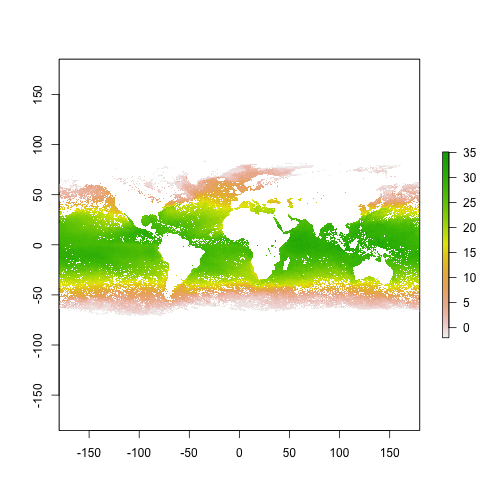
\includegraphics{figure/raster_plot.png}
\caption{plot of chunk raster\_plot}
\end{figure}

\end{document}
